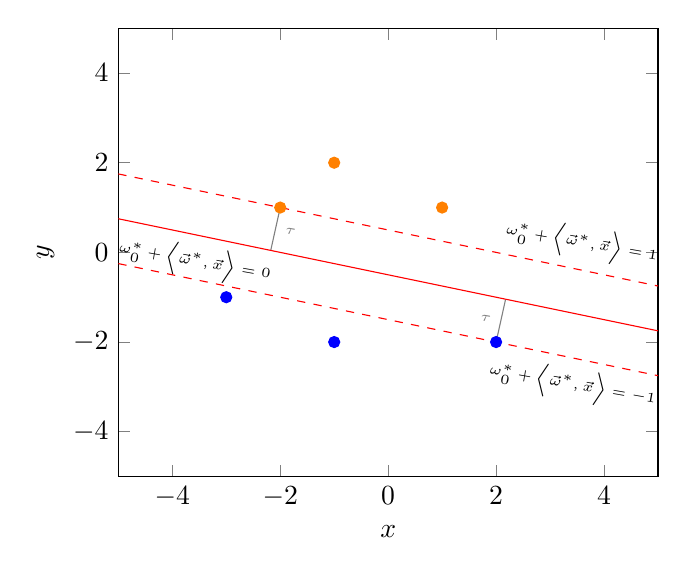
\begin{tikzpicture}

  \begin{axis}[xlabel = $x$, ylabel = $y$, xmin = -5.0, xmax = 5.0, ymin = -5.0, ymax = 5.0]
    
    \addplot[mark = *, , draw = none, color = orange] coordinates {(1,1)}; 
    \addplot[mark = *, , draw = none, color = orange] coordinates {(-1,2)}; 
    \addplot[mark = *, , draw = none, color = orange] coordinates {(-2,1)}; 

    \addplot[mark = *, , draw = none, color = blue] coordinates {(-1,-2)}; 
    \addplot[mark = *, , draw = none, color = blue] coordinates {(2,-2)}; 
    \addplot[mark = *, , draw = none, color = blue] coordinates {(-3,-1)}; 

    \addplot[mark = none, color = gray] coordinates {(-2,1) (-2.175,0.05)} node[right, pos=0.5, rotate=-10] {\tiny$\tau$}; 
    \addplot[mark = none, color = gray] coordinates {(2,-2) (2.175,-1.05)} node[left, pos=0.5, rotate=-10] {\tiny$\tau$}; 

    \addplot[color = red]         {-0.25*x - 0.5} node[below, pos=0.15, rotate=-10] {\color{black}\tiny$\omega_0^* + \left<\vec\omega^*, \vec x\right> = 0$};;
    \addplot[color = red, dashed] {-0.25*x - 1.5} node[below, pos=0.85, rotate=-10] {\color{black}\tiny$\omega_0^* + \left<\vec\omega^*, \vec x\right> = -1$};
    \addplot[color = red, dashed] {-0.25*x + 0.5} node[above, pos=0.85, rotate=-10] {\color{black}\tiny$\omega_0^* + \left<\vec\omega^*, \vec x\right> = 1$};;
    
  \end{axis}

\end{tikzpicture}